\section{Versionskontrolle}
\frame{
	\begin{block}{}
  	\begin{center}
  	\huge{Versionskontrolle}
	\end{center}
  	\end{block}
}			

\subsection*{Was ist Versionskontrolle?}
\frame{
	\frametitle{Was Ist Versionskontrolle?}
	\begin{backgroundblock}{4.5cm}{2.5cm}
		
\includegraphics[width=3.5cm]{img/git_stapel.jpg}
	\end{backgroundblock}
}
\frame{
	\frametitle{Git Branch}
	\begin{backgroundblock}{1cm}{2.5cm}
		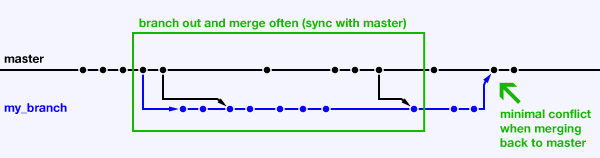
\includegraphics[width=10cm]{img/git_branch.png}
	\end{backgroundblock}
}
\frame{
	\frametitle{Git Workflow}
	\begin{backgroundblock}{1cm}{2.5cm}
		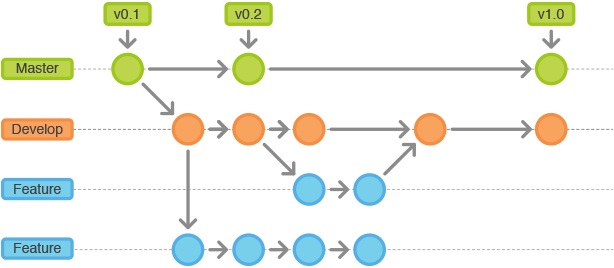
\includegraphics[width=10cm]{img/git_workflow.png}
	\end{backgroundblock}
}
\frame{
	\frametitle{Welche Versionskontrollsystem gibt es?}
	\begin{block}{}
	\begin{itemize}
	\item{Git}
   	\item{Mercurial}
	\item{SVN}
	\item{Andere (2005)}
	\end{itemize}
	\end{block}
}

\frame{
	\frametitle{Welches Versionskontrollsystem ist das richtige?}
	\begin{block}{}
	\begin{itemize}
	\item{Mercurial (code.google.com)}
   	\item{SVN (Probleme, zu alt)}
	\item{Git (github.com - Die Bibliothek von Alexandria des 21. Jahrhunderts)}
	\end{itemize}
	\end{block}
}

\subsection*{Features}
\frame{
	\frametitle{Features von GIT}
	Git ist zentraler Bestandteil jeder modernen IT-Firma.
	\begin{block}{}
	\begin{itemize}
	\item{Kontrolle der Entwicklung/Abrechnung}
   	\item{Motivation}
	\item{Deploy}
	\item{Mehrere Entwickler können an dem selben Projekt arbeiten}
	\item{Backup inklusive Historie}
	\end{itemize}
	\end{block}
}
\frame{
	\frametitle{Projektverlauf visualisiert über Git}
	\begin{backgroundblock}{0.5cm}{2.5cm}
		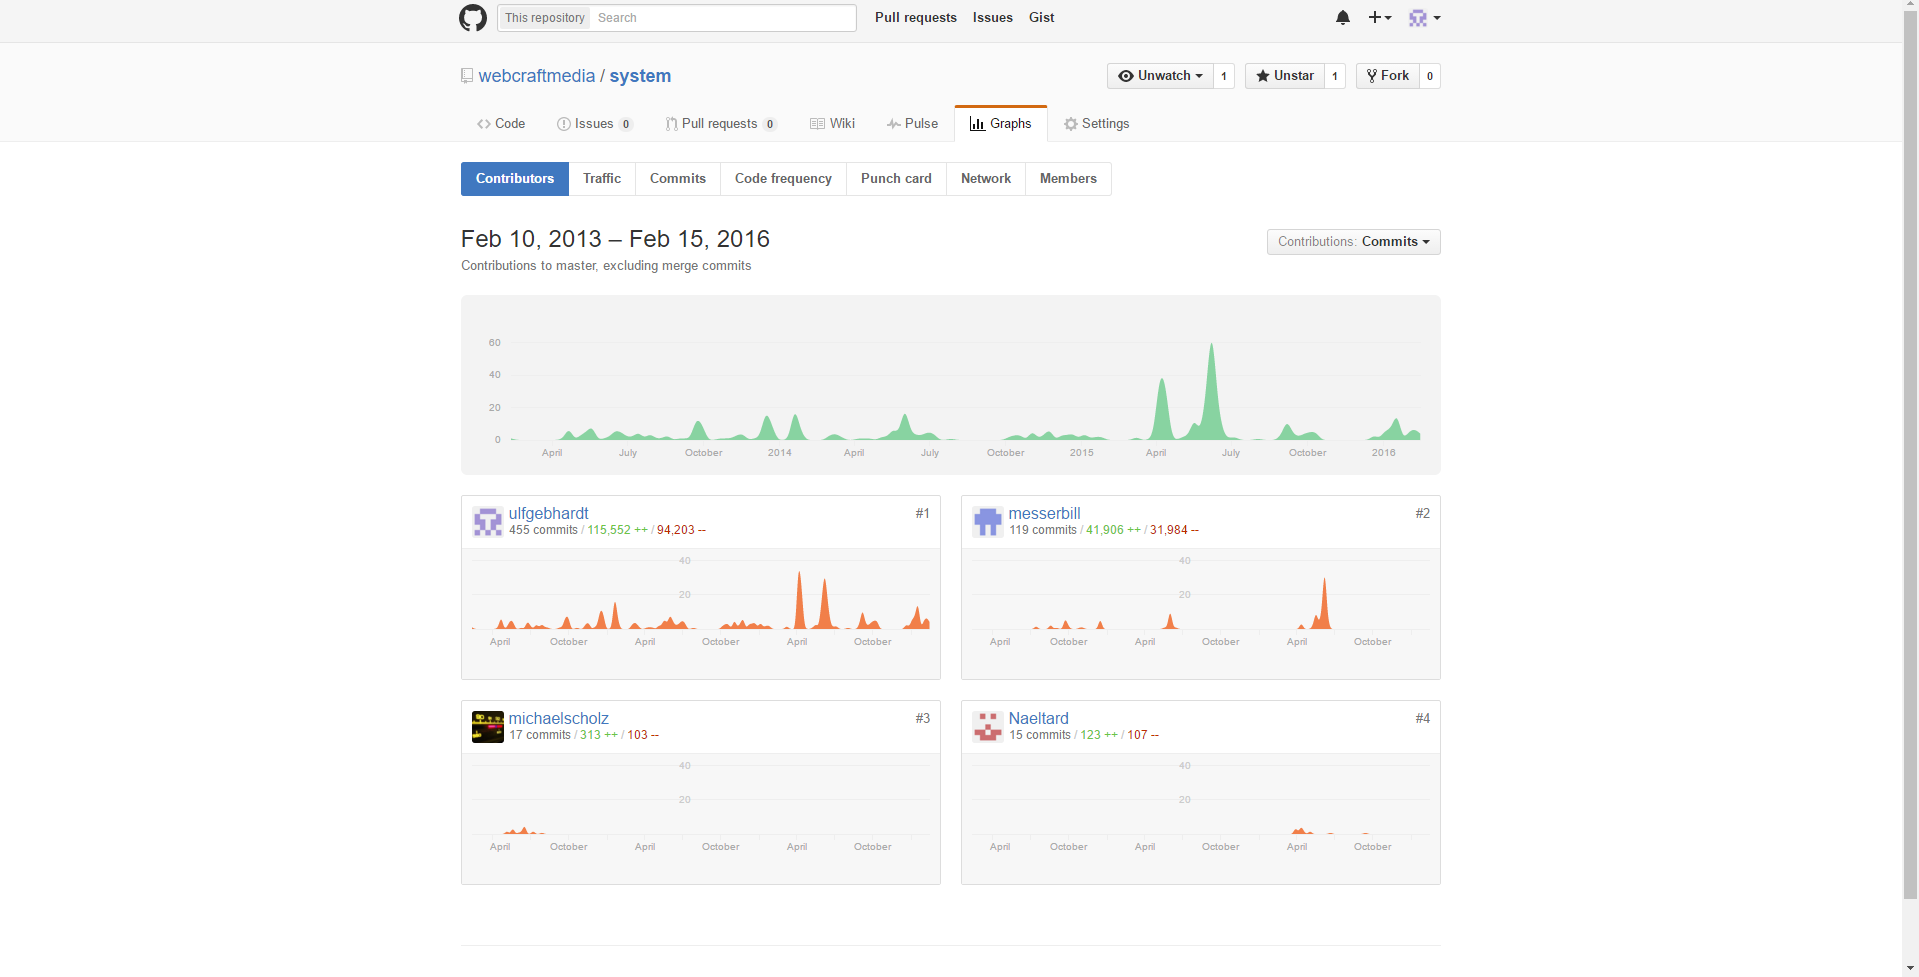
\includegraphics[width=12cm]{img/github_system.png}
	\end{backgroundblock}
}